\documentclass[]{article}
\usepackage{lmodern}
\usepackage{amssymb,amsmath}
\usepackage{ifxetex,ifluatex}
\usepackage{fixltx2e} % provides \textsubscript
\ifnum 0\ifxetex 1\fi\ifluatex 1\fi=0 % if pdftex
  \usepackage[T1]{fontenc}
  \usepackage[utf8]{inputenc}
\else % if luatex or xelatex
  \ifxetex
    \usepackage{mathspec}
  \else
    \usepackage{fontspec}
  \fi
  \defaultfontfeatures{Ligatures=TeX,Scale=MatchLowercase}
\fi
% use upquote if available, for straight quotes in verbatim environments
\IfFileExists{upquote.sty}{\usepackage{upquote}}{}
% use microtype if available
\IfFileExists{microtype.sty}{%
\usepackage{microtype}
\UseMicrotypeSet[protrusion]{basicmath} % disable protrusion for tt fonts
}{}
\usepackage[margin=1in]{geometry}
\usepackage{hyperref}
\hypersetup{unicode=true,
            pdfborder={0 0 0},
            breaklinks=true}
\urlstyle{same}  % don't use monospace font for urls
\usepackage{graphicx,grffile}
\makeatletter
\def\maxwidth{\ifdim\Gin@nat@width>\linewidth\linewidth\else\Gin@nat@width\fi}
\def\maxheight{\ifdim\Gin@nat@height>\textheight\textheight\else\Gin@nat@height\fi}
\makeatother
% Scale images if necessary, so that they will not overflow the page
% margins by default, and it is still possible to overwrite the defaults
% using explicit options in \includegraphics[width, height, ...]{}
\setkeys{Gin}{width=\maxwidth,height=\maxheight,keepaspectratio}
\IfFileExists{parskip.sty}{%
\usepackage{parskip}
}{% else
\setlength{\parindent}{0pt}
\setlength{\parskip}{6pt plus 2pt minus 1pt}
}
\setlength{\emergencystretch}{3em}  % prevent overfull lines
\providecommand{\tightlist}{%
  \setlength{\itemsep}{0pt}\setlength{\parskip}{0pt}}
\setcounter{secnumdepth}{0}
% Redefines (sub)paragraphs to behave more like sections
\ifx\paragraph\undefined\else
\let\oldparagraph\paragraph
\renewcommand{\paragraph}[1]{\oldparagraph{#1}\mbox{}}
\fi
\ifx\subparagraph\undefined\else
\let\oldsubparagraph\subparagraph
\renewcommand{\subparagraph}[1]{\oldsubparagraph{#1}\mbox{}}
\fi

%%% Use protect on footnotes to avoid problems with footnotes in titles
\let\rmarkdownfootnote\footnote%
\def\footnote{\protect\rmarkdownfootnote}

%%% Change title format to be more compact
\usepackage{titling}

% Create subtitle command for use in maketitle
\providecommand{\subtitle}[1]{
  \posttitle{
    \begin{center}\large#1\end{center}
    }
}

\setlength{\droptitle}{-2em}

  \title{}
    \pretitle{\vspace{\droptitle}}
  \posttitle{}
    \author{}
    \preauthor{}\postauthor{}
    \date{}
    \predate{}\postdate{}
  
\usepackage{booktabs}
\usepackage{longtable}
\usepackage{array}
\usepackage{multirow}
\usepackage{wrapfig}
\usepackage{float}
\usepackage{colortbl}
\usepackage{pdflscape}
\usepackage{tabu}
\usepackage{threeparttable}
\usepackage{threeparttablex}
\usepackage[normalem]{ulem}
\usepackage{makecell}
\usepackage{xcolor}

\begin{document}

\hypertarget{dual-inheritance-theory-and-the-origins-of-religious-disbelief}{%
\section{Dual Inheritance Theory and The Origins Of Religious
Disbelief}\label{dual-inheritance-theory-and-the-origins-of-religious-disbelief}}

Will M. Gervais*\textsuperscript{1}, Nava Caluori\textsuperscript{2},
Sarah R. Schiavone\textsuperscript{3}, \& Maxine B.
Najle\textsuperscript{4}

\scriptsize

\textsuperscript{1}Department of Psychology, University of Kentucky

\textsuperscript{2}Department of Psychology, University of Virginia

\textsuperscript{3}Department of Psychology, University of
California-Davis

\textsuperscript{4}Blue Labs Analytics, Washington, D. C.

*Corresponding author. Email:
\href{mailto:will.gervais@gmail.com}{\nolinkurl{will.gervais@gmail.com}}

\hypertarget{preprint-under-review}{%
\subsubsection{PREPRINT under review}\label{preprint-under-review}}

\normalsize
\pagebreak

\hypertarget{abstract}{%
\subsection{Abstract}\label{abstract}}

\textbf{Religion is a core component of human nature, yet a
comprehensive scientific account of religion also needs to account for
religious disbelief. Despite potentially drastic overreporting of
religiosity \#\#, a third of the world's 7 billion human inhabitants may
actually be atheists---merely people who do not believe in God or gods.
The origins of disbelief thus present a key testing ground for theories
of religion. Here, we evaluate the predictions of four theoretical
approaches to the origins of disbelief, and find considerable support
for a dual inheritance (gene-culture coevolutionary) model. Our dual
inheritance model \#\# derives from distinct literatures addressing the
putative 1) core social cognitive faculties that enable mental
representation of gods \#\#, 2) motivational antecedents driving people
to view some god candidates as strategically important \#\#, 3) evolved
cultural learning processes that influence which god candidates naïve
learners treat as real rather than imaginary \#\#, and 4) the intuitive
processes that sustain belief in gods \#\# and the cognitive reflection
that may sometimes undermine it \#\#. We explore the varied origins of
religious disbelief by treating these factors simultaneously in a large
nationally representative (USA, \emph{N} = 1417) dataset with
preregistered analyses. Combined, we find that receiving few cultural
cues of religious commitment is the most potent predictor of religious
disbelief, followed distantly by reflective cognitive style. Additional
exploration suggests that cognitive reflection may primarily predict
reduced religious belief among individuals who witness relatively fewer
credible contextual cues of faith in others. This work empirically
unites four distinct literatures addressing religious belief and
disbelief \#\#, highlights the utility of considering both evolved
cognition and cultural learning in religious transmission \#\#,
emphasizes the dual roles of content-and context-biased social learning,
and sheds light on the shared psychological mechanisms that underpin
both religious belief and disbelief. }

\textbf{Keywords:} atheism; religion; culture; evolution; dual
inheritance theory

\pagebreak

\hypertarget{dual-inheritance-theory-and-the-origins-of-religious-disbelief-1}{%
\section{Dual Inheritance Theory and The Origins Of Religious
Disbelief}\label{dual-inheritance-theory-and-the-origins-of-religious-disbelief-1}}

Religion is somewhat an evolutionary puzzle. Organisms like ants and
aardvarks tend to eschew painful and costly rituals to prove their faith
in unseen ant and aardvark pantheons, respectively. Evolutionary
theories of religion have proliferated in recent years \#\#, and they
make starkly different predictions about the nature and origins of
religious disbelief: some describe atheism as a cognitive deficit \#\#,
others as a mere self-reporting blip unreflective of underlying
cognition \#\#, and yet others as the natural outcome of certain
cultural contexts \#\#. Thus, the origins of disbelief may prove a
crucial testing ground for different theories of religion. Here we test
predictions from four theoretical frameworks (secularization, cognitive
byproduct, cultural evolution, and an emerging dual inheritance
(gene-culture coevolutionary) model of religion \#\# that views both
evolved cognition \#\# and specific cultural learning mechanisms \#\# as
key to the transmission of either faith or atheism \#\#. This work
situates the study of religious disbelief firmly within established
theoretical frameworks for studying the evolution of human behavior and
contributes to broader discussions of the role of transmitted (versus
evoked) culture in core aspects of human nature \#\#.

Religion simultaneously unites and divides like few other aspects of
social life. The sectarian conflicts between groups of religious
believers may obscure a more fundamental schism: that between believers
and atheists. Atheists---merely people who do not believe in the
existence of a God or gods---constitute a large and perhaps growing
proportion of earth's human population \#\#. A prominent estimate from
the opening decade of the current millennium \#\# posits the existence
of 500-700 million atheists. This estimate is in all likelihood a
drastic underestimate \#\#. Atheism prevalence estimates rely on census
and polling data that infer individual beliefs from their self-reports.
However, there is potent anti-atheist stigma that transcends national
and religious boundaries \#\#: even atheists harbor some intuitive moral
distrust of atheists worldwide \#\#. Thus, while it is safe to assume
that self-reported atheists do not believe in God, it is probably also
safe to assume that a great many people privately disbelieve without
openly admitting their atheism. Consistent with this, people routinely
overreport their religious practices \#\#, and indirect measurement of
atheism in the USA reveals a potentially large gulf between some
indirect (\textasciitilde{}26\%) and direct (\textasciitilde{}3\%)
estimates of atheist prevalence \#\#. Combining direct estimates and
inferences drawn from the few available indirect estimates, we predict
that upwards of 2 billion people on earth may in fact be atheists. Many
evolutionary theories of religion posit a universal implicit theism
\#\#, and may thus be fundamentally incompatible with global atheism
that is simultaneously prevalent and deliberately concealed. Therefore,
sustained research into the origins of disbelief is necessary to test
key assumptions of various evolutionary and cultural theories of
religion.

While it is clear that a (perhaps unrecognized) large proportion of the
global population does not believe in gods, what cognitive,
motivational, and cultural factors predict religious disbelief? Distinct
research trajectories have considered the preconditions for sustained
belief in any given god. To currently believe in a god, one 1) must be
able to mentally represent gods, 2) must be motivated to `interact' with
gods, 3) must receive credible cultural cues that some gods are real,
and 4) must intuitively maintain this belief over time. Tweaks to any of
these four components may instead yield disbelief in gods. Separate
lines of research partially support this supposition. First, individual
differences in mentalizing abilities (one key component of mind
perception) predict religious disbelief \#\# in at least some samples
\#\#. Second, although religion flourishes where life is unstable,
existential security predicts reduced religiosity \#\#. Third, lack of
credibility enhancing displays (CREDs) \#\# that one ought to believe in
any gods is a good global predictor of atheism \#\#. Finally, people who
reflectively override their intuitions tend to be less religious than
those who `go with their guts' \#\#, although the magnitude and
consistency of this relation is debatable \#\#. Although these four
factors relate to religious disbelief in isolation, little work
considers their operation in conjunction \#\#.

Different theoretical approaches make divergent predictions about which
of these four factors are the most potent predictors of religious
disbelief. First, secularization models \#\# posit that increases in
existential security (wealth, health, education) reduce religious
motivation; this approach is common in sociology of religion \#\# and in
social psychology, under the banner of compensatory control \#\#.
Second, evolutionary psychology and cognitive science of religion often
view religion as a cognitive byproduct of other mental adaptations \#\#,
such as mind perception or predator detection \#\#. In this view,
challenges in the core cognitive faculties underlying such adaptations
(e.g., mentalizing) would predict disbelief, as would people being able
to override their religious intuitions via cognitive reflection \#\#.
Third, cultural evolutionary models highlight the social learning
processes underpinning religious belief and disbelief, and largely
predict that context-biased social learning such as CREDs would be
strongly associated with degrees of religious belief. Finally, dual
inheritance models somewhat integrate these various perspectives, and
predict that CREDs would be most important, followed by other factors
such as cognitive reflection, mentalizing, and existential security.
Table 1 depicts predictions derived from each of these perspectives. By
simultaneously considering mentalizing, existential security, CREDs, and
cognitive reflection, we are able to evaluate the suitability of each of
these four theoretical approaches for understanding the psychological
origins of religious disbelief.

We preregistered a set of analyses that pit secularization, cognitive
byproduct, socialization, and dual inheritance models against each
other. Specifically, we posed three broad questions:

\begin{enumerate}
\def\labelenumi{\Roman{enumi}.}
\tightlist
\item
  What are the relative contributions of each factor when considered
  simultaneously?
\item
  How do the factors interact with each other in predicting belief and
  disbelief?
\item
  Does early work on each individual factor successfully replicate in a
  nationally representative sample?
\end{enumerate}

To approach these questions, we contracted a nationally representative
sample of USA adults (\emph{N}= 1417) from GfK. Primarily, we were
interested in predicting degrees of religious belief and disbelief with
measures of 1) advanced mentalizing, 2) existential security, 3)
theoretically modeled cues of cultural exposure to credible cues of
religiosity (CREDs), and 4) intuitive versus reflective cognitive style.
For robustness, we also included a number of demographic and
psychological covariates.

Our most important analyses considered the relative contributions of all
four factors operating in concert. As preregistered, we report two
analyses in which the four core factors predict individual differences
in belief and disbelief, both in the presence and absence of additional
covariates. In our full model (see Table 2 and Figure 1), few credible
displays of faith proved to be by far the most powerful predictor of
religious disbelief. Credibility enhancing displays of faith predict
belief, and their absence predicts atheism. Cognitive reflection
remained a consistent predictor of religious disbelief, but following
earlier cross-cultural work \#\# its predictive power was quite meager.
Mentalizing challenges were only weakly associated, if at all, with
disbelief, and existential security predicted essentially nothing.

Next, we probed for interactions between the four factors. Results
suggest an interaction between cultural learning and reflective
cognitive style . We broke down this interaction in two different ways.
First, we considered the association between disbelief and reflective
cognitive style among those comparatively high and low on credible
cultural cues of religious belief (Figure 2a). Reflective cognitive
style primarily predicts religious disbelief among those who were also
comparatively low in cultural exposure to credible religious cues of
faith. Second, we predicted current religious belief from cultural
exposure to credibility enhancing displays of religion and then
correlated reflective cognitive style with the residual. Effectively,
this analysis suggests that reflective thinkers tend to be less
religious than one would assume based solely on their cultural exposure
to religious cues (Figure 2b). It is thus possible that reflective
cognitive style is one mechanism that leads people to lose faith over
time \#\#; in contrast, an intuitive cognitive style leads people to
adhere to their early cultural inputs and perhaps become more religious
in some contexts. These patterns highlight the interactive roles of
cultural context and evolved intuitions on religious cognition, as
predicted by dual inheritance theories.

Finally, we tested each candidate factor in isolation, merely to
replicate previous work. In individual replication analyses (Table 3),
only cultural learning and reflective cognitive style emerged as
consistent predictors of religious disbelief. That two of the candidate
factors culled from existing literature did not appear as robust
predictors in these models may suggest tempered enthusiasm for their
utility as predictors of individual differences in religiosity more
broadly, although they both (especially existential security) may still
be useful in analyzing larger-scale regional and international trends.

Overall, these results present one of the most comprehensive available
analyses of the cognitive, cultural, and motivational factors that
predict individual differences in religious belief and disbelief in the
USA. They also speak directly to competing theoretical models of
religious disbelief, culled from sociology, social psychology,
evolutionary psychology, cognitive science of religion, cultural
evolution, and dual inheritance. Consistent inferences emerged,
suggesting that the most potent predictor of disbelief is---by a wide
margin---lack of exposure to credibility enhancing displays of religious
faith. Once this context-biased cultural learning mechanism is accounted
for, one cognitive factor---a reflective cognitive style---predicts some
people being slightly more prone to religious disbelief than their
cultural upbringing might otherwise suggest. That said, this
relationship was relatively miniscule. Mentalizing and motivational
features did not meaningfully predict belief and disbelief in this
nationally representative sample. Comparing Table 1 and Figure 1, it is
clear that our results are most consistent with dual process theories,
and any model that does not rely heavily on context-biased cultural
learning is likely a poor fit for explaining the origins of religious
disbelief. By extension, such models fail as as evolutionary accounts of
religion.

It is initially puzzling that existential security proved impotent in
our analyses, as it appears to be an important factor in explaining
cross-cultural differences in religiosity. Further, it has proven
successful in experimental work \#\#, although these experimental
insights may be less robust than initially assumed \#\#. It is possible
that our analyses were at the wrong level of analysis to capture the
influence of existential security, which may act as a precursor to other
cultural forces. There may actually be a two-stage generational process
whereby existential security drives down religious behavior in one
generation, leading the subsequent generation to atheism as they do not
witness credibility enhancing displays of faith.

This work suggests two broader meta-scientific points. Of the four
candidate factors we tested, one (credibility enhancing displays) is
derived from formal theoretical modeling in gene-culture coevolution,
while the other three emerged from verbal argumentation. In terms of
predicting large-scale real-world patterns, the formally modeled theory
empirically outclassed the three `veories' . Verbal theorizing is an
important step in the research process, but formal theorizing is an
indispensable tool as well \#\#. Formal models are obviously wrong yet,
they are useful mental prostheses simply because they are precisely and
transparently wrong \#\#. Second, most psychology research nowadays
emerges from convenience samples of undergraduates and Mechanical Turk
workers. These samples are fine for some purposes, but representative
samples are necessary for others. While our nationally representative
sampling allows us to generalize beyond samples we can access for free
(in lab) or cheap (MTurk), even a large nationally representative sample
barely scratches the surface of human diversity \#\#. As such, we
encourage similar analyses across different cultures \#\#. This is
especially necessary because cultural cues themselves emerged as the
strongest predictor of belief and disbelief. If this general pattern
holds across societies, we predict that---beyond religion---veories
developed by WEIRD researchers to explain the weird mental states of
WEIRD participants will continue to ever more precisely answer only an
outlier of an outlier of our most important scientific questions about
human nature.

The importance of transmitted culture and context-biased cultural
learning as a predictor of belief and disbelief cannot be overstated.
Combined, the data we collected suggest that if you are guessing whether
or not individuals are believers or atheists, you are better off knowing
how their parents behaved---did they tithe? Pray regularly? Attend
synagogue?---than how they themselves process information. Further, our
interaction analyses suggest perhaps that sufficiently strong cultural
exposure yields sustained religious commitment, even in the face of the
putatively corrosive influence of cognitive reflection. Theoretically,
these results fit well with dual inheritance theories of religion \#\#,
as evolved cognitive capacities for cultural learning prove to be the
most potent predictor of individual differences in the cross-culturally
universal display of religious belief. In an applied sense, they also
speak to the shared cognitive and cultural forces that generate,
depending on circumstances, either belief or disbelief. Atheists are
becoming increasingly common in the world, not because human psychology
is fundamentally changing, but rather because evolved cognition remains
stable in the face of a rapidly changing cultural context that is itself
the product of a coevolutionary process. Faith emerges in some cultural
contexts, and atheism is the natural result in others.

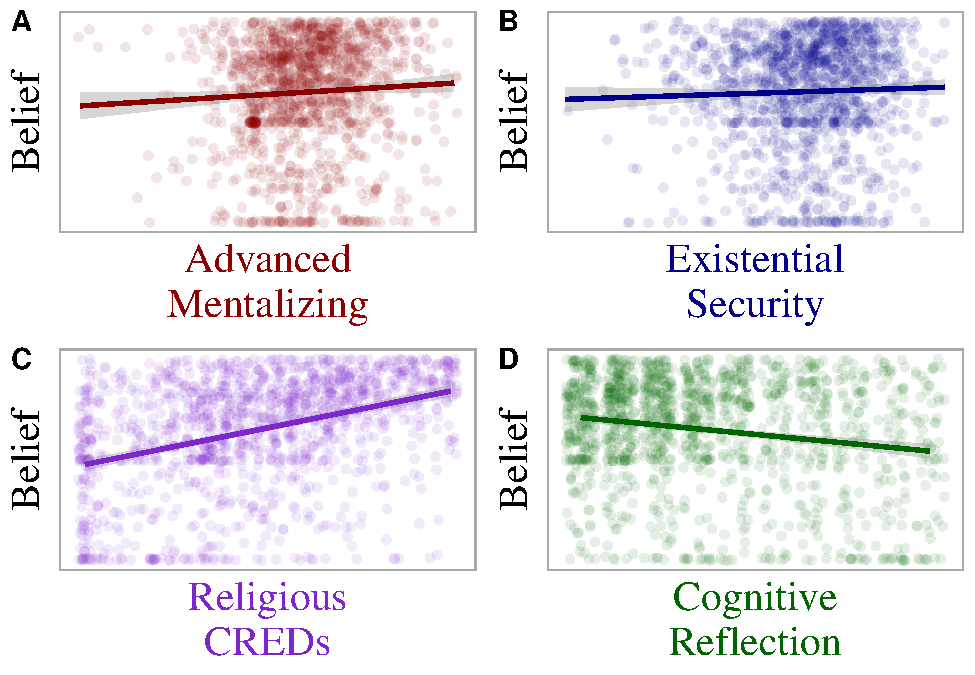
\includegraphics{disbelief-origins-ms_files/figure-latex/individual scatters-1.pdf}

\begin{wraptable}{r}{0pt}
\begin{tabular}{>{\bfseries}l|r|l|l}
\hline
Variable & r & HPDI & Pr\\
\hline
Low Mentalizing & 0.06 & [0, 0.12] & 0.98\\
\hline
Mentalizing (quad) & 0.02 & [-0.02, 0.06] & 0.89\\
\hline
High Security & -0.03 & [-0.09, 0.02] & 0.1\\
\hline
Low CREDs & 0.38 & [0.32, 0.43] & >0.99\\
\hline
High Reflection & 0.18 & [0.12, 0.24] & >0.99\\
\hline
\end{tabular}\end{wraptable}

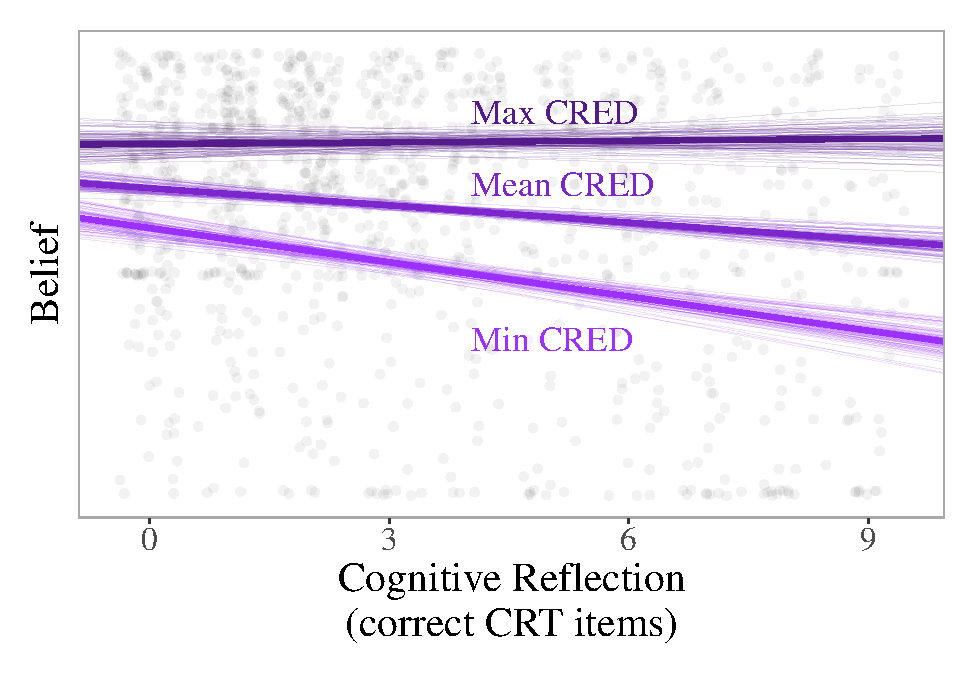
\includegraphics{disbelief-origins-ms_files/figure-latex/interaction plot-1.pdf}

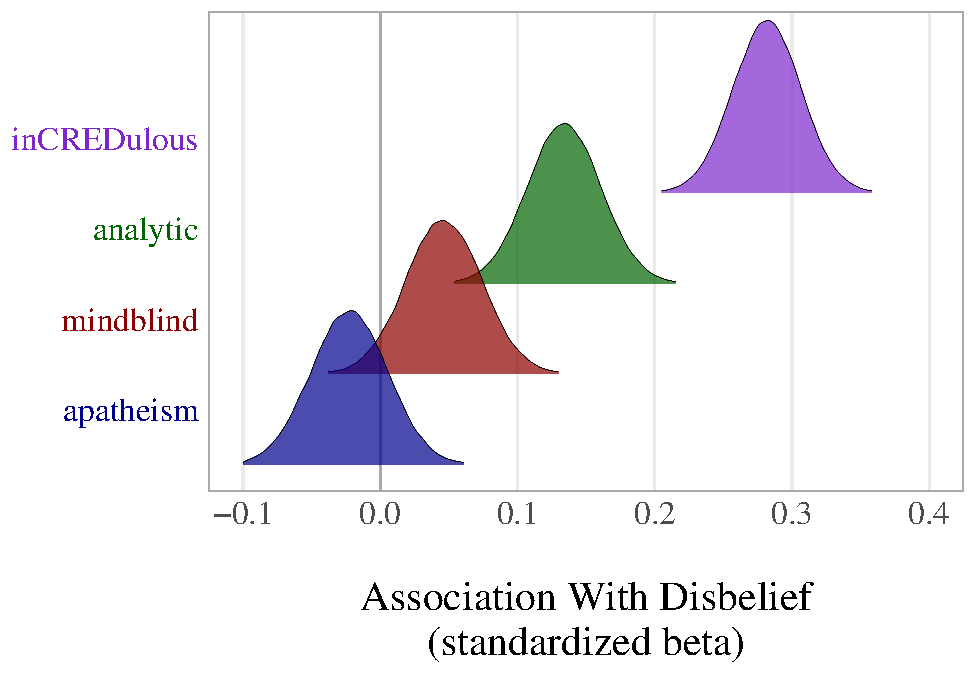
\includegraphics{disbelief-origins-ms_files/figure-latex/posterior plot-1.pdf}

\begin{table}

\caption{\label{tab:full model table}Full Model Summary}
\centering
\begin{tabular}[t]{lrll}
\toprule
Variable & Beta & HPDI & Pr\\
\midrule
Low Mentalizing & 0.05 & [-0.01, 0.11] & 0.95\\
Mentalizing (quad) & 0.01 & [-0.02, 0.04] & 0.81\\
Security & -0.02 & [-0.08, 0.04] & 0.21\\
Low CREDs & 0.28 & [0.23, 0.34] & > 0.99\\
Reflection & 0.13 & [0.08, 0.19] & > 0.99\\
\addlinespace
\hspace{1em}Age & 0.01 & [-0.04, 0.07] & 0.69\\
\hspace{1em}Education & 0.04 & [-0.02, 0.1] & 0.92\\
\hspace{1em}Male & 0.07 & [0.02, 0.13] & > 0.99\\
\hspace{1em}Social Lib & 0.43 & [0.35, 0.52] & > 0.99\\
\hspace{1em}Economic Cons & 0.04 & [-0.05, 0.12] & 0.82\\
\addlinespace
\hspace{1em}Extraversion & 0.02 & [-0.03, 0.08] & 0.82\\
\hspace{1em}Conscientiousness & 0.01 & [-0.04, 0.07] & 0.71\\
\hspace{1em}Neuroticism & 0.00 & [-0.06, 0.07] & 0.56\\
\hspace{1em}Low Agreeableness & 0.10 & [0.04, 0.17] & > 0.99\\
\hspace{1em}Openness & 0.07 & [0.01, 0.13] & > 0.99\\
\addlinespace
\hspace{1em}Honesty/Humility & 0.04 & [-0.02, 0.1] & 0.91\\
\bottomrule
\end{tabular}
\end{table}

\begin{table}

\caption{\label{tab:predictions table}Predictions From Prominent  Theories}
\centering
\begin{tabu} to \linewidth {>{\bfseries}r>{\raggedleft}X>{\raggedleft}X>{\raggedleft}X>{\raggedleft}X>{\raggedleft}X}{>{\bfseries}rrrrrr}
\toprule
Theory & Discipline & Mindblind & Apatheist & inCREDulous & Analytic\\
\midrule
Secularization & Sociology \& Social Psych &  & + + + + &  & \\
Cognitive Byproduct & Ev Psych \& Cog Sci Rel & + + & + &  & + + +\\
Social Learning & Cultural Evolution &  &  & + + + + & \\
Dual Inheritance & Gene-Culture Coevolution & + & indirect & + + + + & +\\
\bottomrule
\end{tabu}
\end{table}


\end{document}
